\documentclass{standalone}
\usepackage{tikz}

\begin{document}

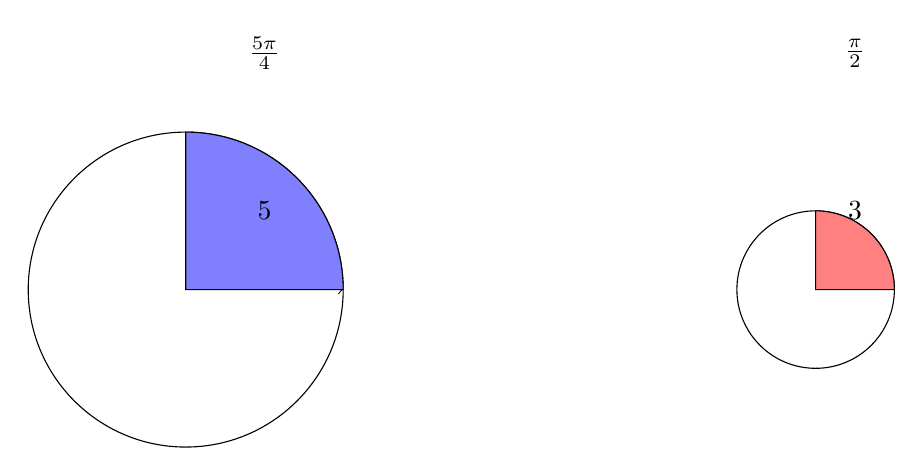
\begin{tikzpicture}[scale=2]

% Large circle
\draw (0,0) circle (1);

% Small circle
\draw (4,0) circle (0.5);

% Line segment
\draw[->] (0,0) -- (1,0);

% Arc for large circle
\draw[fill=blue!50] (0,0) -- (1,0) arc (0:90:1) -- cycle;

% Arc for small circle
\draw[fill=red!50] (4,0) -- (4.5,0) arc (0:90:0.5) -- cycle;

% Labels
\node at (0.5,0.5) {$5$};
\node at (4.25,0.5) {$3$};
\node at (0.5,1.5) {$\frac{5\pi}{4}$};
\node at (4.25,1.5) {$\frac{\pi}{2}$};

\end{tikzpicture}

\end{document}